\frame{
   \frametitle{Que es Thresholding?}
   
    Es una herramienta que nos permite conocer determinadas posiciones de pixeles con el objetivo de efectuar cambios especificos en una imagen.

   \begin{figure}
         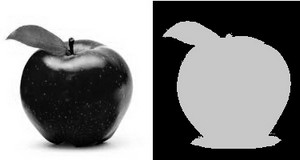
\includegraphics[scale=0.4]{Image/manzana}
   \end{figure}

    Imagen tomada de:
    http://docs.opencv.org/2.4/doc/tutorials/imgproc/threshold/threshold.html
}